% !TEX program = lualatex

\documentclass[
11pt,
captions=tableheading,
%smallheadings,
%headings=big,
headsepline,
footsepline, 
%chapterprefix=false			% weiss nicht was passiert
captions=tableheading,
parskip=half-,
%BCOR=10mm,
%twocolumn, 
%draft
]{scrartcl}

%\usepackage[babelshorthands]{polyglossia}
\usepackage{polyglossia}
\setdefaultlanguage[variant = swiss]{german}

%\usepackage[ngerman]{babel} 
\usepackage[]{ scrlayer-scrpage }
\usepackage[ a4paper,
 total={160mm,244mm},
 left=25mm,
 top=25mm,
 headsep=10mm
 %footsep=12mm
 %,showframe
  ]{geometry}
 \usepackage{fontspec}
\setmainfont{Times New Roman}
\setsansfont{Arial}

\usepackage[dvipsnames]{xcolor}
\usepackage[most]{tcolorbox}
\usepackage[
version=3,
arrows=pgf-filled,
]{mhchem} % für chemische Formeln
\usepackage{microtype}
\usepackage{float}
\usepackage{enumitem}
\usepackage{multicol}
\usepackage{booktabs}
\usepackage{pgfplots}
\usepackage{tabularx}
\usepackage{longtable}
\usepackage{fontawesome5}
\usepackage{pdfpages}

\usepackage{pdflscape} % Für Querformat-Seiten


\usepackage{siunitx}
\usepackage{amsfonts}
\usepackage{tabularx}

%Quellen 
\usepackage[
    backend=bibtex, 
    natbib=true,
    style=numeric,
    sorting=none
]{biblatex}
\addbibresource{../Quellen.bib}

\usepackage[section]{placeins} % avoids images in the wrong section



% order of hyperref, cleverref is important
\usepackage[hidelinks]{hyperref}
\usepackage{cleveref}



\frenchspacing



\floatplacement{figure}{H}

% Labeling of elements
\counterwithin{figure}{section}
\counterwithin{table}{section}
\counterwithin{equation}{section}

% Colors
\definecolor{blau_bauschule}{RGB}{22,65,148}

% Titel mit Bauschule blau gemäss CI manual
\addtokomafont{section}{\color{blau_bauschule}\Huge}
\addtokomafont{subsection}{\color{blau_bauschule}\huge}
\addtokomafont{subsubsection}{\color{blau_bauschule}\Large}
\addtokomafont{paragraph}{\normalsize}
\addtokomafont{subparagraph}{\small}
% Pagestyle
\pagestyle{scrheadings}
\ihead{\fontsize{9pt}{2pt}\selectfont }
\ohead{\fontsize{9pt}{2pt}\selectfont Baustoffe}
\chead{\fontsize{9pt}{2pt}\selectfont \headmark}
\ifoot{\fontsize{9pt}{2pt}\selectfont Bauschule Aarau} 
\ofoot{\fontsize{9pt}{2pt}\selectfont \thepage} %Seitennummer
\cfoot{\fontsize{9pt}{2pt}\selectfont }
\setkomafont{pagehead}{\normalfont}
\setkomafont{pagefoot}{\normalfont}
\setkomafont{pagefoot}{\normalfont}
\setkomafont{pagehead}{\normalfont}
\setkomafont{pagefoot}{\normalfont}
\setcounter{topnumber}{1}
\setcounter{bottomnumber}{1}
\automark[section]{subsection}


% Bild- und Tabellenunterschriften
\renewcommand*{\figurename}{Abbildung}
\renewcommand*{\tablename}{Tabelle}


% Titel
\title{Baustoffe}
%\author{Patrick Pfändler}
\date{2021}

% https://tex.stackexchange.com/questions/501018/how-to-write-a-minitoc-with-plain-koma-script

%https://www.mrunix.de/forums/archive/index.php/t-74962.html


\makeatletter
\newcommand\reaction@[1]{\begin{equation}\ce{#1}\end{equation}}
\newcommand\reaction@nonumber[1]%
{\begin{equation*}\ce{#1}\end{equation*}}
\newcommand\reaction{\@ifstar{\reaction@nonumber}{ \reaction@}}
\makeatother
%renewtagform{reaction}[R ]{(}{)}

%% Custom icons 
\newcommand{\Lerniziel}{\faBullseye}
\newcommand{\Diskussion}{\faComments}
\newcommand{\TR}{\faCalculator}
\newcommand{\Fragen}{\faQuestionCircle}
\newcommand{\LeherTafel}{\faChalkboardTeacher}








\begin{document}


\pagestyle{scrheadings}

% Commands
\newcommand{\myNmm}[1]
{
\sisetup{per-mode=symbol}
\SI{#1}{\newton\per\mm\squared}
}


\newcommand{\kommzerielleProdukte}[1]
{
    \textcolor{Brown}{Kommerzielle Produkte:}  #1
}




%\renewcommand{\familydefault}{\sfdefault}
%\setkomafont{captionlabel}{\itshape \fontsize{10pt}{2pt}}
%\setkomafont{caption}{\sffamily} 

\newtcolorbox{Definition}[1]{
colback=green!5!white,
colframe=green!75!black,fonttitle=\bfseries,
title=#1}


\newtcolorbox{Merke}{
enhanced,
boxrule=0pt,frame hidden,
borderline west={4pt}{0pt}{red!75!black},
colback=white,
sharp corners
}

\newtcolorbox{Masseinheit}[1]{
enhanced,
boxrule=1pt,colframe=blue,
colback=white,
sharp corners, 
colframe=blue!75!black,
title = #1, 
after title={\hfill\colorbox{ NavyBlue}{Masseinheit}}
}

\newtcbox{\ExampleSimple}[1][gray]{on line,
arc=0pt,outer arc=0pt,colback=#1!10!white,%colframe=#1!50!black,
frame hidden,
boxsep=0pt,left=1pt,right=1pt,top=1pt,bottom=1pt,
boxrule=0pt,bottomrule=1pt,toprule=1pt}

%\maketitle
{\color{blau_bauschule}\fontsize{30pt}{21pt}\selectfont \textbf{Dokumentierter Unterrichtsbesuch}}





\section*{Übersicht}

\begin{table}[ht]
    \centering
    \label{tab:uebersicht}
    \begin{tabularx}{\textwidth}{@{}Xp{11cm}@{}}
    \toprule
    Lehrperson: & Patrick Pfändler \\
    Studiengang: & HFP Bauführung \\
    Fach: & Baustoffe \\
    \midrule
    Klasse: & HTf-26 \\
    Semester: & 1 \\
    Anzahl Schüler: & 14 \\
    Ort: & Bauschule Aarau \\
    Datum: & 16.12.2024 \\
    Uhrzeit: & 08:00 - 10:00 \\
    Unterrichtszeit: & 2 Stunden \\
    Schulzimmer: & 301 \\
    Schulzimmerausrüstung: & Beamer (2x), Hellraumprojekterersatz, Flipchart \\
    \midrule
    Persönliche Ausrüstung: & Laptop, Pointer, IPad \\
    \midrule
    Inhalt der Lektion: & Wiederholung der wichtigsten Themen des Fachs Baustoffe und Feedbackrunde \\
    \bottomrule
    \end{tabularx}
    \end{table}



\clearpage
\vspace*{2cm}
\setcounter{tocdepth}{3} % Tiefe des Inhaltverzeichnisses steuern
\tableofcontents%
\clearpage

\subsection*{Abkürzungsverzeichnis}
\begin{table}[H]
    \centering
    \label{tab:abkuerzungen}
    \begin{tabularx}{\textwidth}{@{}ll@{}}
    \toprule
    %\midrule
    Bsp. & Beispiel \\
    LP & Lehrperson \\
    SF & Sozialform \\
    FK & Fachkompetenz \\
    \bottomrule
    \end{tabularx}
    \end{table}



\clearpage

\section{Bedigungsanalyse}

\subsection{Zielgruppenanalyse}
%Input von Roberto folgt
Folgt noch.

\subsection{Rahmenbedingungen}
\subsubsection{Strukturelle Rahmenbedingungen}
Das Zeitbudget für die Unterrichtszeit beträgt 2 Stunden. Der Unterricht findet in der Bauschule Aarau statt. Die Schülerzahl beträgt 14 Personen. Der Unterricht beginnt um 08:00 Uhr und endet um 10:00 Uhr.
Die Lektion startet überlicherweise im Schulzimmer.

Die Studierenden haben eine fixes Schulzimmer zugeteilt und eine fixe Sitzordnung. Der Lehrerpult befindet sich vorne in der Mitte des Raumes. Der Beamer ist an der Decke montiert und kann über ein Kabel mit dem Laptop verbunden werden. Ein Hellraumprojektor ist ebenfalls vorhanden. Ein Flipchart steht zur Verfügung.


Die Studierenden arbeiten in der Regel mit einem Laptop und einem Tablet. Einzelne Studiererende drucken die Unterlagen aus. 
Für einige Aufgaben wird ein Taschenrechner vorausgesetzt.

\subsection{Jahresplanung}
Für das Fach Baustoffe stehen rund \SI{64}{\hour} Unterrichtszeit zur Verfügung.
Diese Lektion ist die letzte Doppelstunde im Fach Baustoffe. 
Weitere Lektionen bei dieser Klasse sind erst im Jahr 2025 geplant. 
Die genannten Lektionen sollen dann spezifisch auf die HFP Prüfung vorbereiten. Aktuell gibt es leider keine Musterprüfungen für die HFP Prüfung. Diese wurden 2024 erwartet, sind aber noch nicht verfügbar.

\subsection{Berufspädaogisches Konzept}
\subsubsection{Kognitive Taxonomiestufen nach Bloom}

\begin{table}[H]
    \centering
    \label{tab:Bloom}
    \caption{Kognitive Taxonomiestufen nach Bloom \cite{bloom1956taxonomy}, adaptiert von \cite{BerufspädagogischesKonzept_BauschuleAarau}.}
    \begin{longtable}{@{}llp{12cm}@{}}
        \toprule
        \textbf{Stufen} & \textbf{Begriff} & \textbf{Beschreibung} \\ 
        \midrule
        K1 & Wissen & Sie geben gelerntes Wissen wieder und rufen es in gleichartiger Situation ab. \\ 
        K2 & Verstehen & Sie erklären oder beschreiben gelerntes Wissen in eigenen Worten. \\ 
        K3 & Anwenden & Sie wenden gelernte Technologien/Fertigkeiten in unterschiedlichen Situationen an. \\ 
        K4 & Analyse & Sie analysieren eine komplexe Situation, d.h. sie gliedern Sachverhalte in Einzelelemente, decken Beziehungen zwischen Elementen auf und finden Strukturmerkmale heraus. \\ 
        K5 & Synthese & Sie kombinieren einzelne Elemente eines Sachverhalts und fügen sie zu einem Ganzen zusammen. \\ 
        K6 & Beurteilen & Sie beurteilen einen mehr oder weniger komplexen Sachverhalt aufgrund von bestimmten Kriterien. \\ 
        \bottomrule
    \end{longtable}
\end{table}




\subsubsection{RITA-Modell}
\begin{table}[H]
    \centering
    \label{tab:RITA_Modell}
    \caption{RITA-Modell, adaptiert von \cite{BerufspädagogischesKonzept_BauschuleAarau}.}
    \begin{tabularx}{\textwidth}{@{}Xp{11cm}@{}}
    \toprule
    %\midrule
    R:  & Ressourcen aktivieren \\
    I: & Informationen verarbeiten \\
    T: & Transfer anbahnen \\
    A: & Auswerten \\
    \bottomrule
    \end{tabularx}
    \end{table}


\clearpage


\section{Lektionsplanung}
\subsection{Fachliche Grundlagen}
Die Studierenden hatten über \SI{60}{\hour} das Fach Baustoffe. 
Sämtliche Themen wurden bereits abgehandelt, sowohl formativ als auch summativ geprüft. 



\subsection{Lernziele}
\subsubsection{Fachkompetenzen}
Die Studierenden repetieren die wichtigsten Themen des Fachs Baustoffe.
Die Lernziele \faBullseye\, für die einzelnen Themen sind den Studierenden bekannt.



\subsection{Sozialform}
Die Sozialform ist Frontalunterricht. Die Studierenden sitzen im Schulzimmer und hören der Lehrperson zu. Es wird auf eine aktive Beteiligung der Studierenden geachtet.

\subsection{Medieneinsatz}
Der Beamer wird für die Präsentation der Lerninhalte verwendet. Ein Hellraumprojektor steht als Ersatz zur Verfügung. Ein Flipchart wird für die Visualisierung von Inhalten bei Bedarf verwendet.

\subsection{Grobplanung}
Die folgenden Lerninhalte werden in der Lektion behandelt:
\begin{itemize}
    \item Wiederholung der wichtigsten Themen des Fachs Baustoffe
    \item Beantwortung von Fragen der Studierenden
    \item Ausblick auf die HFP Prüfung
    \item Feedbackrunde
\end{itemize}




\begin{landscape}
\subsection{Verlaufsplanung}
\begin{longtable}{@{}lp{10cm}p{8cm}l@{}}
    \toprule
    \textbf{Zeit} & \textbf{Aktivität der Lehrperson} & \textbf{Aktivitäten der Studierenden} & \textbf{Medieneinsatz} \\ 
    \midrule
    08:00 - 08:05 & \textbf{Einstieg:}Begrüssung der Studierenden und Vorstellung von Natalie Räber; Anschliessend vorstellen des Programms; Abholen, ob Fragen zur Lektionsunterricht bestehen; Webuntis: Erfassen der Absenzen; Skizzieren des Stundenablaufs & Begrüssung der Lehrperson und vorbereiten der Unterlagen; Hören der LP zu. & Beamer mit PP-Folien\\
    \midrule
    09:55 - 10:00 & \textbf{Abschluss:} Zusammenfassung der wichtigsten Punkte des Jahres; Verabschiedung der Studierenden & Zusammenpacken der Unterlagen und Verabschiedung der LP & Beamer mit PP-Folien\\
    \bottomrule
\end{longtable}
\end{landscape}
\clearpage

\begin{landscape}
    
    \section{Reflexion}
    \subsection{Selbstreflexion}
    \begin{table}[H]
        \centering
        \label{tab:Relexion}
        \caption{Kognitive Taxonomiestufen nach Bloom \cite{bloom1956taxonomy}, adaptiert von \cite{BerufspädagogischesKonzept_BauschuleAarau}.}
        \begin{longtable}{@{}p{10cm}|p{13cm}@{}}
            \toprule
            Didaktische Entscheidungen reflektieren, Zielerreichung analysieren, Optimierungsbedarf benennen und begründen & {} \\
            \midrule
            Planung und Durchführung vergleichen und Abweichungen differenziert begründen. & {} \\
            \midrule
            Eigenes Handeln als Lehrperson im Hinblick auf das Lernen der Schülerinnen und Schüler reflektieren, Handlungsalternativen entwickeln und begründen. & {} \\
            \midrule
            Entwicklungsziele und nächste Schritte formulieren und begründen.   & {} \\
            \bottomrule
        \end{longtable}
    \end{table}
\end{landscape}
    





\clearpage
\addcontentsline{toc}{section}{Literatur}

\printbibliography
\clearpage
\section*{Anhang}
\addcontentsline{toc}{section}{Anhang}

\subsection*{Grobplanung}
\addcontentsline{toc}{subsection}{Grobplanung}

\clearpage
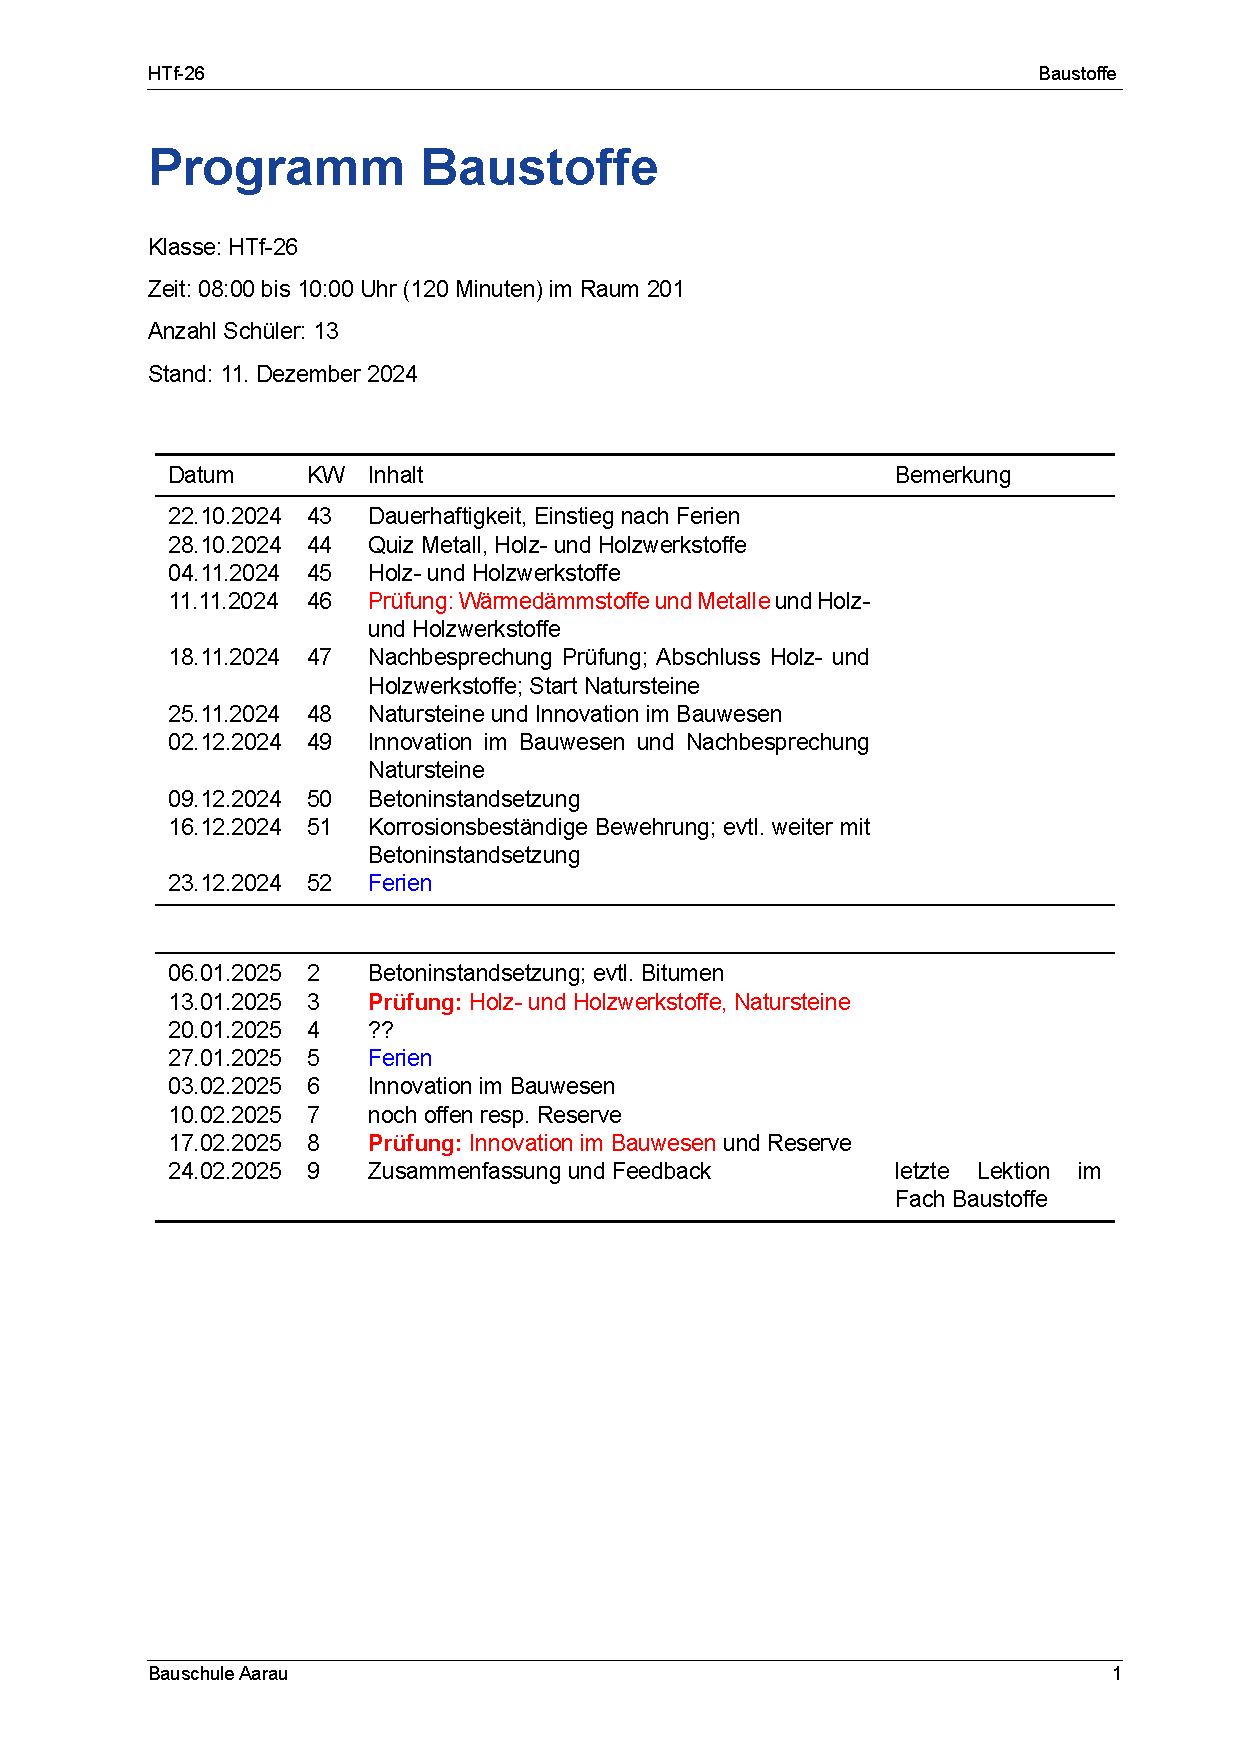
\includepdf[pages=-]{../../HTf-26/Programm/Programm_HTf-26.pdf}

\section*{Lernziele}
\addcontentsline{toc}{subsection}{Lernziele}

Beispiel von Lernzielen einer Prüfung:
\clearpage
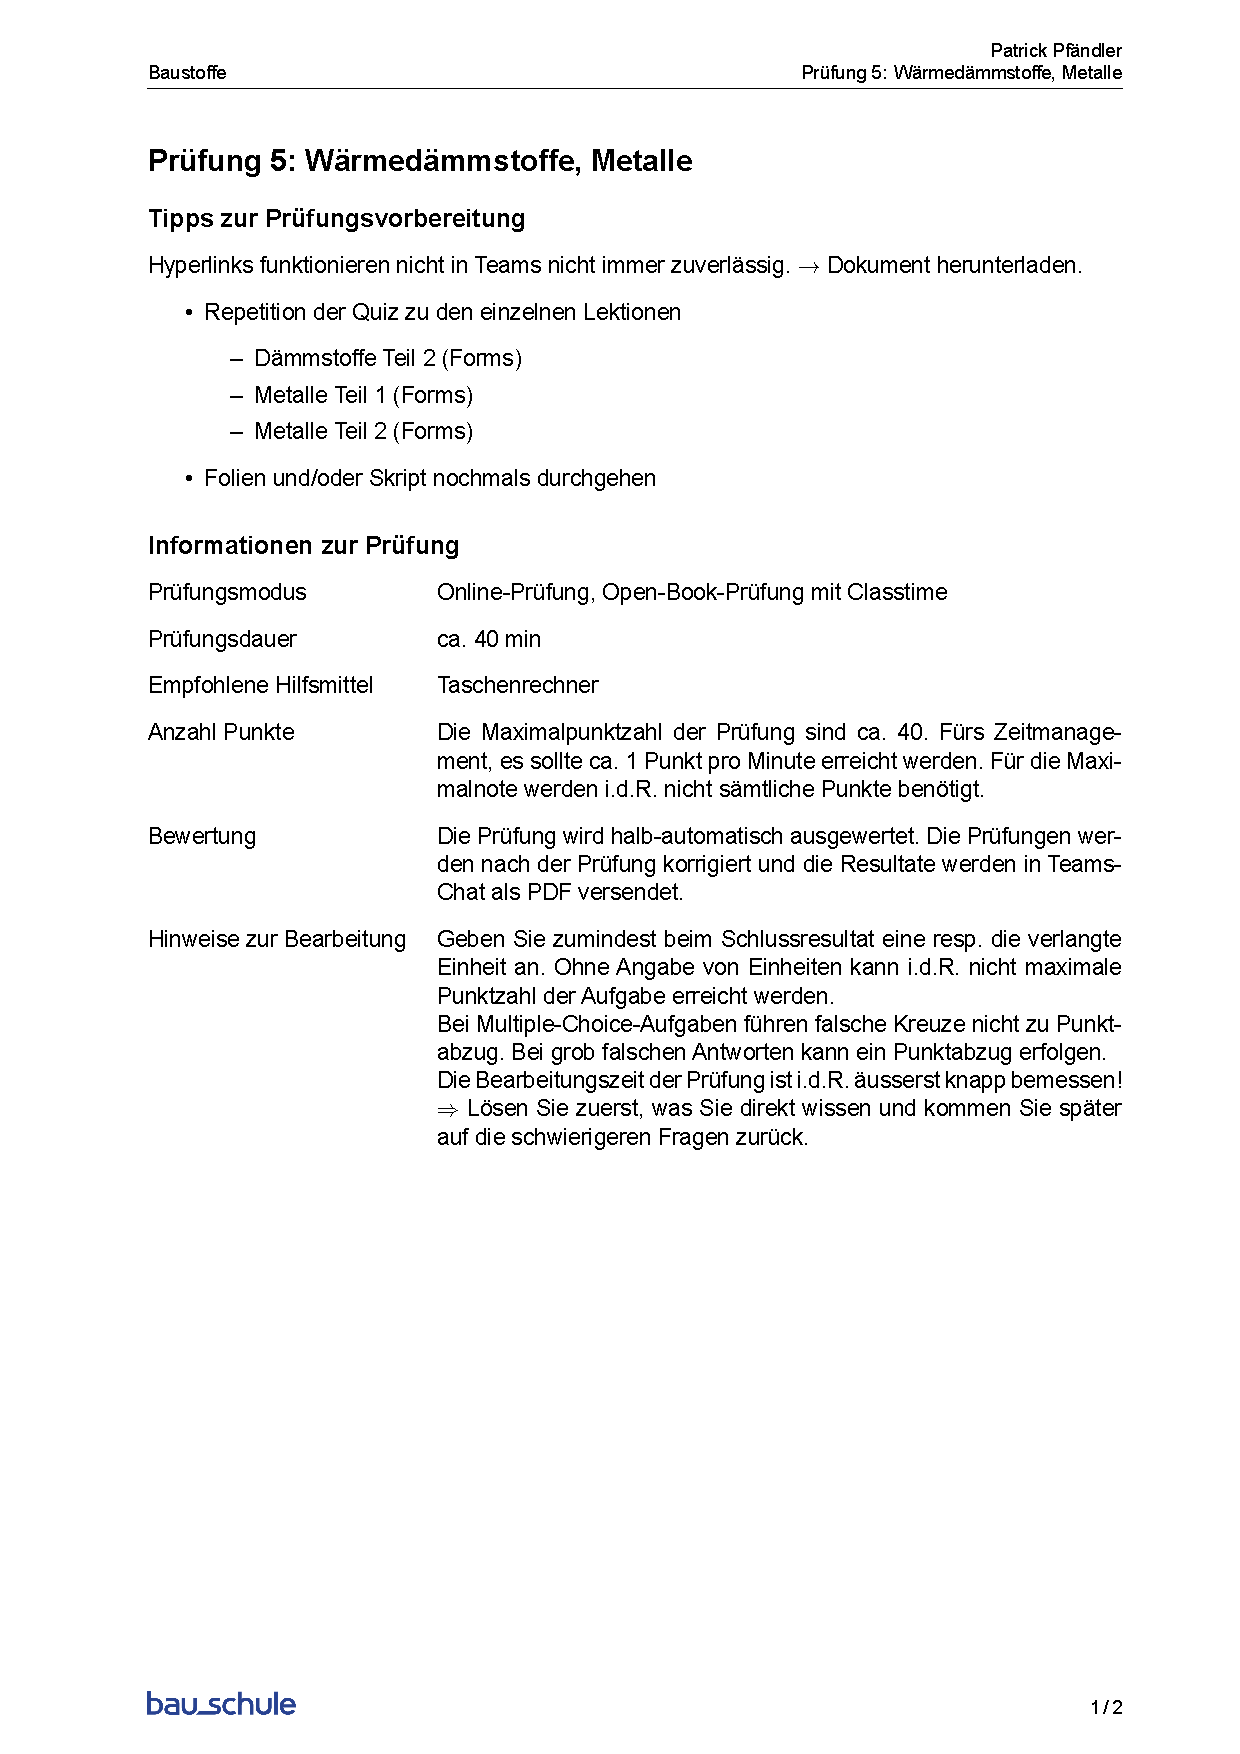
\includepdf[pages=-]{../..//HTf-26/WDS_Metall/Pr5_WDS_Metalle_Lernziele.pdf}





\end{document}